%%%%%%%%%%%%%%%%%%%%%%%%%%%%%%%%%%%%%%%%%%%%%%%%%%%%%%%%%%%%%%%%%%%%%%%%%%
%
%    DD-ERS.tex  (use only for JWST Director's Discretionary Early Release Science proposals)
%
%
%
%    JAMES WEBB SPACE TELESCOPE 
%    OBSERVING PROPOSAL TEMPLATE 
%    FOR CYCLE 1 DD-ERS (2017)
%
%    Version 1.0 May 2017.
%
%    Guidelines and assistance
%    =========================
%     Cycle 1 Announcement Web Page:
%
%         https://jwst-docs.stsci.edu/display/JSP/JWST+Cycle+1+Proposal+Opportunities
%
%    Please contact the JWST Help Desk if you need assistance with any
%    aspect of your proposal:
%    	    http://jwsthelp.stsci.edu
%
%
%
%%%%%%%%%%%%%%%%%%%%%%%%%%%%%%%%%%%%%%%%%%%%%%%%%%%%%%%%%%%%%%%%%%%%%%%%%%%

% The template begins here. Please do not modify the font size from 12 point.

\documentclass[12pt]{article}
\usepackage{jwstproposaltemplate}
\usepackage{hyperref}
\usepackage{graphicx}

%\setlength {\textwidth}{180mm} 


\usepackage{enumitem}
%%\usepackage{deluxetable}
%\usepackage{graphicx,fancyhdr,natbib,subfigure}
\usepackage{epsfig, epsf}
\usepackage{amsmath, cancel, amssymb}
\usepackage{lscape, longtable, caption}
\usepackage{dcolumn}% Align table columns on decimal point
\usepackage{bm}% bold math
\usepackage{hyperref, ifthen, multicol}
\usepackage{verbatim}
\usepackage{color}
\usepackage[usenames,dvipsnames]{xcolor}
%% http://en.wikibooks.org/wiki/LaTeX/Colors



%%%%%%%%%%%%%%%%%%%%%%%%%%%%%%%%%%%%%%%%%%%
%       define Journal abbreviations      %
%%%%%%%%%%%%%%%%%%%%%%%%%%%%%%%%%%%%%%%%%%%
\def\nat{Nat} \def\apjl{ApJ~Lett.} \def\apj{ApJ}
\def\apjs{ApJS} \def\aj{AJ} \def\mnras{MNRAS}
\def\prd{Phys.~Rev.~D} \def\prl{Phys.~Rev.~Lett.}
\def\plb{Phys.~Lett.~B} \def\jhep{JHEP} \def\nar{NewAR}
\def\npbps{NUC.~Phys.~B~Proc.~Suppl.} \def\prep{Phys.~Rep.}
\def\pasp{PASP} \def\aap{Astron.~\&~Astrophys.} \def\araa{ARA\&A}
\def\jcap{\ref@jnl{J. Cosmology Astropart. Phys.}}%
\def\physrep{Phys.~Rep.}

\newcommand{\preep}[1]{{\tt #1} }

%%%%%%%%%%%%%%%%%%%%%%%%%%%%%%%%%%%%%%%%%%%%%%%%%%%%%
%              define symbols                       %
%%%%%%%%%%%%%%%%%%%%%%%%%%%%%%%%%%%%%%%%%%%%%%%%%%%%%
\def \Mpc {~{\rm Mpc} }
\def \Om {\Omega_0}
\def \Omb {\Omega_{\rm b}}
\def \Omcdm {\Omega_{\rm CDM}}
\def \Omlam {\Omega_{\Lambda}}
\def \Omm {\Omega_{\rm m}}
\def \ho {H_0}
\def \qo {q_0}
\def \lo {\lambda_0}
\def \kms {{\rm ~km~s}^{-1}}
\def \kmsmpc {{\rm ~km~s}^{-1}~{\rm Mpc}^{-1}}
\def \hmpc{~\;h^{-1}~{\rm Mpc}} 
\def \hkpc{\;h^{-1}{\rm kpc}} 
\def \hmpcb{h^{-1}{\rm Mpc}}
\def \dif {{\rm d}}
\def \mlim {m_{\rm l}}
\def \bj {b_{\rm J}}
\def \mb {M_{\rm b_{\rm J}}}
\def \mg {M_{\rm g}}
\def \qso {_{\rm QSO}}
\def \lrg {_{\rm LRG}}
\def \gal {_{\rm gal}}
\def \xibar {\bar{\xi}}
\def \xis{\xi(s)}
\def \xisp{\xi(\sigma, \pi)}
\def \Xisig{\Xi(\sigma)}
\def \xir{\xi(r)}
\def \max {_{\rm max}}
\def \gsim { \lower .75ex \hbox{$\sim$} \llap{\raise .27ex \hbox{$>$}} }
\def \lsim { \lower .75ex \hbox{$\sim$} \llap{\raise .27ex \hbox{$<$}} }
\def \deg {^{\circ}}
%\def \sqdeg {\rm deg^{-2}}
\def \deltac {\delta_{\rm c}}
\def \mmin {M_{\rm min}}
\def \mbh  {M_{\rm BH}}
\def \mdh  {M_{\rm DH}}
\def \msun {M_{\odot}}
\def \z {_{\rm z}}
\def \edd {_{\rm Edd}}
\def \lin {_{\rm lin}}
\def \nonlin {_{\rm non-lin}}
\def \wrms {\langle w_{\rm z}^2\rangle^{1/2}}
\def \dc {\delta_{\rm c}}
\def \wp {w_{p}(\sigma)}
\def \PwrSp {\mathcal{P}(k)}
\def \DelSq {$\Delta^{2}(k)$}
\def \WMAP {{\it WMAP \,}}
\def \cobe {{\it COBE }}
\def \COBE {{\it COBE \;}}
\def \HST  {{\it HST \,\,}}
\def \Spitzer  {{\it Spitzer \,}}
\def \ATLAS {VST-AA$\Omega$ {\it ATLAS} }
\def \BEST   {{\tt best} }
\def \TARGET {{\tt target} }
\def \TQSO   {{\tt TARGET\_QSO}}
\def \HIZ    {{\tt TARGET\_HIZ}}
\def \FIRST  {{\tt TARGET\_FIRST}}
\def \zc {z_{\rm c}}
\def \zcz {z_{\rm c,0}}

\newcommand{\ltsim}{\raisebox{-0.6ex}{$\,\stackrel
        {\raisebox{-.2ex}{$\textstyle <$}}{\sim}\,$}}
\newcommand{\gtsim}{\raisebox{-0.6ex}{$\,\stackrel
        {\raisebox{-.2ex}{$\textstyle >$}}{\sim}\,$}}
\newcommand{\simlt}{\raisebox{-0.6ex}{$\,\stackrel
        {\raisebox{-.2ex}{$\textstyle <$}}{\sim}\,$}}
\newcommand{\simgt}{\raisebox{-0.6ex}{$\,\stackrel
        {\raisebox{-.2ex}{$\textstyle >$}}{\sim}\,$}}

\newcommand{\Msun}{M_\odot}
\newcommand{\Lsun}{L_\odot}
\newcommand{\lsun}{L_\odot}
\newcommand{\Mdot}{\dot M}

\newcommand{\sqdeg}{deg$^{-2}$}
\newcommand{\lya}{Ly$\alpha$\ }
%\newcommand{\lya}{Ly\,$\alpha$\ }
\newcommand{\lyaf}{Ly\,$\alpha$\ forest}
%\newcommand{\eg}{e.g.~}
%\newcommand{\etal}{et~al.~}
\newcommand{\lyb}{Ly$\beta$\ }
\newcommand{\cii}{C\,{\sc ii}\ }
\newcommand{\ciii}{C\,{\sc iii}]\ }
\newcommand{\civ}{C\,{\sc iv}\ }
\newcommand{\SiIV}{Si\,{\sc iv}\ }
\newcommand{\mgii}{Mg\,{\sc ii}\ }
\newcommand{\feii}{Fe\,{\sc ii}\ }
\newcommand{\feiii}{Fe\,{\sc iii}\ }
\newcommand{\caii}{Ca\,{\sc ii}\ }
\newcommand{\halpha}{H\,$\alpha$\ }
\newcommand{\hbeta}{H\,$\beta$\ }
\newcommand{\hgamma}{H\,$\gamma$\ }
\newcommand{\hdelta}{H\,$\delta$\ }
\newcommand{\oi}{[O\,{\sc i}]\ }
\newcommand{\oii}{[O\,{\sc ii}]\ }
\newcommand{\oiii}{[O\,{\sc iii}]\ }
\newcommand{\heii}{[He\,{\sc ii}]\ }
\newcommand{\nv}{N\,{\sc v}\ }
\newcommand{\nev}{Ne\,{\sc v}\ }
\newcommand{\neiii}{[Ne\,{\sc iii}]\ }
\newcommand{\aliii}{Al\,{\sc iii}\ }
\newcommand{\siiii}{Si\,{\sc iii}]\ }


\begin{document}


\clearpage
%%%%%%%%%%%%%%%%%%%%%%%%%%%%%%%%%%%%%%%%%%%%%%%%%%%%%%%%%%%%%%%%%%%%%%%%%%%

%   1. RATIONALE FOR DD ERS Program
%       (see https://jwst-docs.stsci.edu/display/JSP/JWST+DD+ERS+Proposal+Preparation)
%
%
\rationaletime          % Do not delete this command.
% Enter your rationale for selection as a DD ERS program.
\vspace{-4pt}
\section*{{\sc Executive Summary}}

\vspace{-6pt}
\noindent
{\it 1. Justification for ERS time}\\
Our Director’s Discretionary time for an Early Release Science
(DD-ERS) program will help the community learn about the longest
wavelength spectrograph on the {\it James Webb Space Telescope
(JWST)}, the Mid-Infrared Instrument (MIRI) Medium-resolution
spectrometer (MRS).  We will release a suite of science-enabling
products (SEPs) via a public data analysis and code repository that we
have already begun to build: \href{https://github.com/miri-mrs}{\tt
github.com/miri-mrs}.  The accompanying documentation is also already
being written: \href{http://miri-mrs.readthedocs.io/}{{\tt
miri-mrs.readthedocs.io}}.  {\it Our primary SEP goal is to produce a
Python package that quickly manipulates and analyzes the full MRS
Level 3 data, in particular the MRS Spectral Cubes and 1D spectra.}

\smallskip \smallskip \smallskip
\noindent
{\it 2. Project Management Plan \& Budget} \\
Our team members have a long and proven history of delivering SEPs,
catalogs, data products, web access pages, documentation and the
necessary helpdesk support for large collaborations on strict
deadlines.  Our project is led by a STFC Ernest Rutherford Senior
Research Fellow, who is able to contribute 100\% FTE to achieving the
major science goals of the proposal, as well as leading the initial
development of the SEPs. We also ask for support for two postdoctoral
researchers who will be in place at Launch time.

\smallskip \smallskip \smallskip
\noindent
{\it 3. Scientific Justification}\\
Our science case is straight-forward, yet strikes at the heart of a
major and still open extragalactic astrophysical question: {\it What
are the star-formation properties of mid-infrared luminous quasars at
the peak of quasar activity? } We will answer this by looking for the
presence of polycyclic aromatic hydrocarbon (PAH) spectral features in
$z\approx2.5$ infrared bright quasars.  Furthermore, we will use the
IFU capability of MIRI MRS in order to quantify the spatial location
of the IR luminosity. This is an ideal investigation for {\it James
Webb}; no other current or near-future facility, ground or
space-based, has the combination of MIR spectroscopy, angular
resolution and the sensitivity required for accessing the PAH spectral
features at $z>2$, {\it and} being able to spatial resolve their
structure.


\smallskip 
\smallskip \smallskip
\noindent
{\it 4. Description of the Targets}\\
We have four primary targets; all are available for early observation.
We also have a back-up list of ten secondary targets, any of which
would allow us to achieve our SEP and Science goals. These fourteen
objects have extensive associated multiwavelength data with our four
primary targets known to exhibit interesting kinematic behavior.

\smallskip 
\smallskip \smallskip
\noindent
{\it 5. Team Diversity}\\
Our team is an ensemble of observational extragalactic experts with a
broad geographical dispersion. This is a new collaboration, but with
substantial heritage and expertise from the SDSS, the {\it
HST/Chandra} Deep Field surveys, and more recent ground-based IR IFU
collaborations (e.g., VLT/KMOS).  

\section*{Science Rationale}
\vspace{-6pt}
\noindent
Over 50 years after their formal identification, and over two decades
since the calculation of their space density evolution, several
fundamental facts remain unknown for high-luminosity AGN,
i.e. quasars: What is the main AGN triggering mechanism at the height
of quasar activity at redshifts $z=2-3$? What direct observational
evidence in individual objects links AGN activity to star formation?
Can we observe ``AGN feedback'' in action, in situ, for the most
luminous sources at their peak activity?  Such unknowns about the
co-evolution of black holes and their host galaxies remain among the
most fundamental unanswered questions in extragalactic astronomy.  And
they will be answered with the launch of the {\it James Webb Space
Telescope}.

\smallskip \smallskip
\noindent
Our team has identified a population of obscured, mid-infrared bright
quasars at the peak of cosmological quasar activity.  These sources
are mid-IR luminous and may be powered by major bursts of star
formation tied to an early phase of galaxy
evolution/formation. However, their global star-formation properties
are currently unknown.  Observations with {\it JWST} MIRI, and in
particular MRS spectroscopy, will quantify the level of star-formation
in these objects.  {\it We will observe four ``extremely red'' quasars
with MIRI MRS across the full wavelength range to high signal to
noise.} These observations will address the fundamental question of
the link between star-formation and AGN activity, by quantifying and
studying the morphological and kinematic properties for both of these
processess; an investigation {\it JWST} was specifically built for.

\smallskip \smallskip
\noindent
It is unknown whether the large IR luminosities observed in these
quasars is from star formation, which would produce strong polycyclic
aromatic hydrocarbon (PAH) spectral features, or, if it is from the hot
dust near the central quasar, which should produce much weaker/no PAH
emission (due to the AGN MIR emission diluting and even destroying PAH
features). {\it Via the detection, or otherwise, of PAH spectral
features, we will measure the SFRs during what is potentially a very
early/obscured stage of massive galaxy formation in the extremely red
quasar population.}

\smallskip \smallskip
\noindent
MIRI MRS is the instrument of choice since no other spectrometer on
{\it JWST} observes longward of 5.3$\mu$m; going redder than this is
crucial in order to detect PAH features in $z>2$ objects.  If present
we will observe the most prominent, well-known major PAH emission
features at 3.3, 6.2, 7.7, and 8.6$\mu$m. The mid-IR spectral region
also presents a suite of high-ionization lines and critically, we will
have access to the \nevi 7.65$\mu$m line which can be used to measure
the instantaneous luminosity of the central engine.  {\it The desire
to immediately gain high signal-to-noise spectra in order to
investigate the physics and chemistry of quasar PAHs, along with
observational overhead concerns, pushes us to observe each object for
3.59 hours, for a total program Charged Time of 22.20 hours.}


\section*{Community Access Rationale}
\vspace{-6pt}
\noindent
We have already begun to design and create science-enabling products
(SEPs) to help the community understand JWST's capabilities.  Our MIRI
MRS Repo \href{https://github.com/miri-mrs}{{\tt github.com/miri-mrs}}
is active and completely accessible to anyone in the broader
community.  The accompanying documentation is also already being
written: \href{http://miri-mrs.readthedocs.io/}{{\tt
miri-mrs.readthedocs.io}}.  {\it Our primary SEP goal is to produce a
Python package that quickly manipulates and analyzes the full MRS
Level 3 data, in particular the MRS Spectral Cubes and 1D spectra. }
We note there is already Python legacy code for this type of analysis:
\href{https://spectral-cube.readthedocs.io/}{\tt
spectral-cube.readthedocs.io}. Critically, we have
already begun working closely with the MIRI team (due to the P.I.'s
location at Edinburgh) and will continue to develop tools here for the
MIRI MRS.

\smallskip \smallskip
\noindent
Our timeline has delivery of the first set (`beta') of MIRI MRS SEPs
before the Cycle 1 GO Deadline (March 2018); our v1.0.0 (with
e.g. MIRSim mock data) before the launch of JWST (October 2018) and
then rapid version updates once the start of science operations
commences in April 2019.

\smallskip \smallskip
\noindent
Our team's commitment to an open access ideology, not only for data,
but for analysis codes, documentation, and scientific manuscripts is
already evident and in place, for an example, see the P.I.'s GitHub
\href{https://github.com/d80b2t}{{\tt /github.com/d80b2t}}.  
%%
%%
%%
We are thus extremely well-placed to satisfy the overall goals of the
DD ERS program.

\medskip \medskip
\medskip \medskip




\clearpage
%%%%%%%%%%%%%%%%%%%%%%%%%%%%%%%%%%%%%%%%%%%%%%%%%%%%%%%%%%%%%%%%%%%%%%%%%%%

%   2. SCIENTIFIC JUSTIFICATION
%       (see https://jwst-docs.stsci.edu/display/JSP/JWST+DD+ERS+Proposal+Preparation)
%
%
\justification          % Do not delete this command.
% Enter your scientific justification here. 
\newcommand{\imw}{$i$--$W3$}
\newcommand{\imwf}{$i$--$W4$}
\newcommand{\rmwf}{$r$--$W4$}
\newcommand{\imwt}{$i$--$W2$}
\newcommand{\wtmwf}{$W3$--$W4$}
%\newcommand{\kms}{km s$^{-1}$}
\newcommand{\cmN}{cm$^{-2}$}
\newcommand{\cmn}{cm$^{-3}$}
\newcommand{\msun}{M$_{\odot}$}
\newcommand{\lsun}{L$_{\odot}$}
\newcommand{\lam}{$\lambda$}
\newcommand{\mum}{$\mu$m}
\newcommand{\ebv}{$E(B$$-$$V)$}
\newcommand{\heii}{\mbox{He\,{\sc ii}}}
\newcommand{\cv}{\mbox{C\,{\sc v}}}
\newcommand{\civ}{\mbox{C\,{\sc iv}}}
\newcommand{\ciii}{\mbox{C\,{\sc iii}}}
\newcommand{\cii}{\mbox{C\,{\sc ii}}}
\newcommand{\nv}{\mbox{N\,{\sc v}}}
\newcommand{\niv}{\mbox{N\,{\sc iv}}}
\newcommand{\niii}{\mbox{N\,{\sc iii}}}
\newcommand{\ovii}{\mbox{O\,{\sc vii}}}
\newcommand{\ovi}{\mbox{O\,{\sc vi}}}
\newcommand{\ov}{\mbox{O\,{\sc v}}}
\newcommand{\oiv}{\mbox{O\,{\sc iv}}}
\newcommand{\oiii}{\mbox{O\,{\sc iii}}}
\newcommand{\oii}{\mbox{O\,{\sc ii}}}
\newcommand{\oi}{\mbox{O\,{\sc i}}}
\newcommand{\feii}{\mbox{Fe\,{\sc ii}}}
\newcommand{\feiii}{\mbox{Fe\,{\sc iii}}}
\newcommand{\mgii}{\mbox{Mg\,{\sc ii}}}
\newcommand{\neviii}{\mbox{Ne\,{\sc viii}}}
\newcommand{\aliii}{\mbox{Al\,{\sc iii}}}
\newcommand{\siiv}{\mbox{Si\,{\sc iv}}}
\newcommand{\siiii}{\mbox{Si\,{\sc iii}}}
\newcommand{\siii}{\mbox{Si\,{\sc ii}}}
%\newcommand{\lya}{\mbox{Ly$\alpha$}}
%\newcommand{\lyb}{\mbox{Ly$\beta$}}
\newcommand{\hi}{\mbox{H\,{\sc i}}}

\newcommand{\imw}{$i$--$W3$}
\newcommand{\imwf}{$i$--$W4$}
\newcommand{\rmwf}{$r$--$W4$}
\newcommand{\imwt}{$i$--$W2$}
\newcommand{\wtmwf}{$W3$--$W4$}
%\newcommand{\kms}{km s$^{-1}$}
\newcommand{\cmN}{cm$^{-2}$}
\newcommand{\cmn}{cm$^{-3}$}
\newcommand{\msun}{M$_{\odot}$}
\newcommand{\lsun}{L$_{\odot}$}
\newcommand{\lam}{$\lambda$}
\newcommand{\mum}{$\mu$m}
\newcommand{\ebv}{$E(B$$-$$V)$}
\newcommand{\heii}{\mbox{He\,{\sc ii}}}
\newcommand{\cv}{\mbox{C\,{\sc v}}}
\newcommand{\civ}{\mbox{C\,{\sc iv}}}
\newcommand{\ciii}{\mbox{C\,{\sc iii}}}
\newcommand{\cii}{\mbox{C\,{\sc ii}}}
\newcommand{\nv}{\mbox{N\,{\sc v}}}
\newcommand{\niv}{\mbox{N\,{\sc iv}}}
\newcommand{\niii}{\mbox{N\,{\sc iii}}}
\newcommand{\ovii}{\mbox{O\,{\sc vii}}}
\newcommand{\ovi}{\mbox{O\,{\sc vi}}}
\newcommand{\ov}{\mbox{O\,{\sc v}}}
\newcommand{\oiv}{\mbox{O\,{\sc iv}}}
\newcommand{\oiii}{\mbox{O\,{\sc iii}}}
\newcommand{\oii}{\mbox{O\,{\sc ii}}}
\newcommand{\oi}{\mbox{O\,{\sc i}}}
\newcommand{\feii}{\mbox{Fe\,{\sc ii}}}
\newcommand{\feiii}{\mbox{Fe\,{\sc iii}}}
\newcommand{\mgii}{\mbox{Mg\,{\sc ii}}}
\newcommand{\neviii}{\mbox{Ne\,{\sc viii}}}
\newcommand{\aliii}{\mbox{Al\,{\sc iii}}}
\newcommand{\siiv}{\mbox{Si\,{\sc iv}}}
\newcommand{\siiii}{\mbox{Si\,{\sc iii}}}
\newcommand{\siii}{\mbox{Si\,{\sc ii}}}
%\newcommand{\lya}{\mbox{Ly$\alpha$}}
%\newcommand{\lyb}{\mbox{Ly$\beta$}}
\newcommand{\hi}{\mbox{H\,{\sc i}}}


One lasting scientific legacy of the {\it Hubble Space Telescope
(HST)} will be the discovery of giant black holes at the centers of
galaxies, confirming the longstanding theory of the ``central
engines'' of quasars. One of the major surprises from the {\it Hubble}
was the discovery of a correlation between black hole mass and galaxy
properties.  This connection, causal or otherwise may provide crucial
clues to how and why these black holes formed and how their host
galaxies evolved. As of the launch of the {\it James Webb Space
Telescope (JWST), this is one of the outstanding questions in
astrophysics.}
%%Assessment of Options for Extending the Life of the Hubble Space Telescope: Final Report (2005)
%% https://www.nap.edu/read/11169/chapter/5

Furthermore, discovery of spectral lines in active galaxies reveals that black holes can trigger massive star formation. 
As such, %the two main energy sources available to a galaxy are nuclear fusion in stars and gravitational accretion onto compact objects. 
%%
The link between massive galaxies and the central super-massive black holes (SMBHs) that seem ubiquitous in them is now thought to be vital to the understanding of galaxy formation and evolution ([1], [2]).  As such, huge observational and theoretical effort has been invested in trying to measure and understand the physics involved in these enigmatic systems.\\

\smallskip
\smallskip
\noindent
Hubble (more or less) discovered $M-\sigma$. \\
Gives rise to the idea of AGN/QSO feedback (in order to shape the LF at the high-mass end)\\
However, {\it direct observational evidence} for AGN feedback is conspicuous by its absence. This is especially true at high-$z$, e.g. $z=2-3$, at the height of the Quasar Epoch. \\
We have identified the best candidates that suggest we are seeing quasar feedback in action, in situ at high-redshift. These are the ``Extremely Red Quasars'' identified via their WISE W3/4 colors. \\
As such, these milliJansky luminous AGN {\it are ideal targets for JWST MIRI}. 




\medskip
\medskip

\smallskip
\smallskip
\noindent
{\bf \underline{The Extremely Red Quasar Population}:}
By matching the quasar catalogues of the Sloan Digital Sky Survey
(SDSS), the Baryon Oscillation Spectroscopic Survey (BOSS) to the
Wide-Field Infrared Survey Explorer (WISE), Ross et al. (2015)
discovered quasars with extremely red infrared-to-optical colours:
$r_{\rm AB}-W4_{\rm Vega}>14$ mag, i.e., $F_\nu({\rm 22\mu
m})/F_\nu(r) \gtrsim 1000$.  These objects have infrared luminosities
$\sim 10^{47}$ erg s$^{-1}$.  The original motivation here was to look
for PAHs that had redshifted in the WISE W4 band for $z\approx$2.5
quasars in order to study and link luminous AGN activity and star
formation at the ``height of the quasar epoch''.

Hamann et al. (2017) then fully and properly refined the selection of
the ERQs, changed the definition based on other data and common
properties, and indeed found many more objects in this new scheme. The
ERQs have a suite of peculiar emission-line properties including large
rest equivalent widths (REWs), unusual ``wingless'' line profiles,
large \nv /\lya , \nv /\civ , \siiv /\civ\ and other flux ratios, and
very broad and blueshifted [\oiii ] \lam 5007.

In Hamann et al., our team identified a ``core'' sample of 97 ERQs
with nearly uniform peculiar properties selected via \imw\ $\ge 4.6$
(AB) and REW(\civ ) $\ge$ 100 \AA\ at redshifts 2.0--3.4. A broader
search finds 235 more red quasars with similar unusual
characteristics. The core ERQs have median luminosity $\left<\log L
({\rm ergs/s})\right> \sim 47.1$, sky density 0.010 deg$^{-2}$,
surprisingly flat/blue UV spectra given their red UV-to-mid-IR colors,
and common outflow signatures including BALs or BAL-like features and
large \civ\ emission-line blueshifts. Their SEDs and line properties
are inconsistent with normal quasars behind a dust reddening
screen. These ``Core ERQs'' are a unique obscured quasar population
with extreme physical conditions related to powerful outflows across
the line-forming regions. Patchy obscuration by small dusty clouds
could produce the observed UV extinctions without substantial UV
reddening.


\smallskip
\smallskip
\noindent
In Zakamska et al. (2016) we used XShooter/VLT to measure rest-frame
optical spectra of four $z\sim 2.5$ extremely red quasars. We
discovered very broad (full width at half max$= 2600-5000$ km
s$^{-1}$), strongly blue-shifted (by up to 1500 km s$^{-1}$)
\oiii$\lambda$5007\AA\ emission lines in these objects. In a large
sample of type 2 and red quasars, \oiii kinematics are positively
correlated with infrared luminosity, and the four objects in our
sample are on the extreme end both in \oiii kinematics and infrared
luminosity.
%%
As such, we estimate that at least 3\% of the bolometric luminosity in
these objects is being converted into the kinetic power of the
observed wind. Photo-ionization estimates suggest that the \oiii
emission might be extended on a few kpc scales, which would suggest
that the extreme outflow is affecting the entire host galaxy of the
quasar. These sources may be the signposts of the most extreme form of
quasar feedback at the peak epoch of galaxy formation, and may
represent an active ``blow-out'' phase of quasar evolution. 


\smallskip
\smallskip
\noindent
Alexandroff et al. (2017 submitted and in prep.).... \\



\medskip
\medskip
\smallskip
\smallskip
\noindent
{\bf \underline{MIR spectroscopy}:}
Fom Veilleux arXiv:0201118v1:: 
How do galaxies form? How do they evolve? How do supermassive black holes fit in this picture of galaxy formation? Which objects are the main contributors to the overall energy budget of the universe? To prop- erly answer these questions, one will need to differentiate objects powered by nuclear fusion in stars (i.e. normal and starburst galaxies) from objects pow- ered by mass accretion onto supermassive black holes (quasars and AGNs). A wide variety of diagnostic tools have been used in the past for this purpose with different degree of success.

Direct spectroscopy searches for the presence of the broad recombination lines at wavelengths where the effects of dust extinction are reduced.
We follow ``Veilleux's Commandments'':
\begin{itemize}
\item Thou shalt use lines which emphasize the differences between H II regions and AGNs; i.e., use high-ionization lines or low-ionization lines produced in the partially ionized zone. 
\item Thou shalt use strong lines which are easy to measure in typical spectra.
\item Thou shalt avoid lines which are badly blended with other emission or absorption line features.
\item Thou shalt use lines with small wavelength separation to minimize sensitivity to reddening.
\item Thou shalt use line ratios from the same elements or involving hydrogen recombination lines to eliminate or reduce abundance dependence.
\item Thou shalt avoid lines from Mg, Si, Ca, Fe – depleted onto dust grains. 
%\item Thou shalt use lines easily accessible to current UV/optical/IR detectors. 
\item Thou shalt avoid lines affected by strong stellar absorption features. 
\item Thou shalt avoid lines affected by strong atmospheric features.
\item Thou shalt use lines at long wavelengths to reduce the effects of dust extinction.
\end{itemize}


{\bf From Padovani et al.,  arXiv:1707.07134v1}
%%3.4 MIR spectroscopy
IR spectroscopy, particularly with the InfraRed Spectro- graph (IRS;
Houck et al. 2004) on board the Spitzer Space Telescope, provided new
insights into the physics and classi- fication of AGN. The unambiguous
observations of the sil- icate feature at 9.7 μm in emission in many
known AGN (Hao et al., 2005; Siebenmorgen et al., 2005; Sturm et al.,
2005; Buchanan et al., 2006; Shi et al., 2006) came as the long sought
confirmation of the unified scheme. At the same time, however, IRS
observations indicated that in some cases the source of obscuration
resides in the host rather than the torus (e.g. Goulding et al., 2012;
Hatziminaoglou et al., 2015).  Identification through MIR spectroscopy
is very pow- erful, allowing to detect obscured AGN components even
when the MIR is dominated by the host galaxy. Several clas- sification
diagrams have been developed to determine the AGN contribution to an
observed spectrum based on cer- tain spectral features, such as high
ionisation emission lines like \nev, \neii and \oiv, the EW of
PAH features and the strength of the silicate feature at 9.7 μm (see,
e.g. Spoon 21 panstarrs.stsci.edu/ et al., 2007; Armus et al., 2007;
Veilleux et al., 2009; Hernán-Caballero \& Hatziminaoglou, 2011). A
number of techniques have also been developed to model the observed
MIR spec- tra and constrain the AGN and starburst contributions (see
e.g. Schweitzer et al., 2008; Nardini et al., 2008; Deo et al., 2009;
Feltre et al., 2013).  Although MIR spectroscopy has had a great
impact on our understanding of AGN, the number of objects studied
through these techniques is limited when compared to pho- tometric
studies, as spectroscopic observations require sig- nificantly longer
integration times. Ground-based observa- tions are generally limited
to the brightest targets due to the effects of the Earth’s atmosphere
(e.g. Alonso-Herrero et al., 2016), while deeper observations were
possible with the IRS during its cryogen-cooled phase. For the most
part, such observations were limited to z 1 luminous IR galaxies
(LIRGs), ultraluminous IR galaxies (ULIRGs), and quasars (Hernan-Caballero \& Hatziminaoglou, 2011, and references therein) although a
number of higher redshift ULIRGs were also studied by IRS (see
e.g. Kirkpatrick et al., 2012). The impact of these techniques will be
greatly expanded by the upcoming JWST (Gardner et al. 2006) and Space
Infrared Telescope for Cosmology and Astrophysics (SPICA; Naka- gawa
et al. 2015), that will probe significantly fainter targets and will
allow us to select new, currently inaccessible, sets of objects, as
discussed next.


\medskip
\medskip
\smallskip
\smallskip
\noindent
{\bf \underline{Polycyclic Aromatic Hydrocarbons}:}
Polycyclic Aromatic Hydrocarbons (PAHs) are abundant, ubiquitous, and
a dominant force in the interstellar medium of galaxies (see e.g.,
Tielens, 2008, ARAA, 46, 289 for a review).  Aromatic features are
already a significant component of dusty galaxy spectra as early as
$z\approx2$ (Yan et al., 2005, ApJ, 628, 604).  and the infrared (IR)
emission features at 3.3, 6.2, 7.7, 8.6, and 11.3 $\mu$m are generally
attributed to IR fluorescence from (mainly) far-ultraviolet (FUV)
pumped large polycyclic aromatic hydrocarbon (PAH) molecules. As such,
these features trace the FUV stellar flux and are thus a measure of
star formation (Peeters et al, 2004, ApJ, 613, 986).
%%
Given the redshift of our ERQs and the MIRI wavelength coverage we will coverage $1.36 \leq \lambda_{\rm emitted} \leq 8.6 \mu$m.


\medskip
\medskip
\smallskip
\smallskip
\noindent
{\bf \underline{Relation to Spitzer IRS}:}
Major Achievement of Spitzer was IRS. \\
$R\sim600$, now $R\sim2000s$, which allows {\it chemistry.}\\
Spitzer IRS died before WISE; therefore now WISE W4 objects were observed by the IRS.\\
i.e. no $z\sim2.5$ ERQs w/ feedback in action were observed. \\




%\clearpage
\iffalse
Comparison to Spitzer IRS (as much for NPRs guide than anything!!) 
\begin{table}
\begin{center}
\begin{tabular}{ || l | c | c  || }
\hline\hline 
                                     & Spizter IRS     & JWST MRS \\
\hline
Wavelength /$\mu$m     & 5.2 -- 38   & 5.0 -- 28.5 \\
\hline\hline 
\end{tabular}
\end{center}
\end{table}
\fi


\medskip
\medskip
\smallskip
\smallskip
\noindent
{\bf \underline{MIRI Imaging}:}
Imaging of the ERQs will tell us what environments they live in (currently totally unknown).\\
Just look at the ERQs: flux from central source $\Rightarrow$ AGN; flux from extended 
$\Rightarrow$ SF; Big puzzle since Spitzer (e.g. and cf. the submm population). \\



\medskip
\medskip
\smallskip
\smallskip
\noindent
{\bf \underline{Next Steps}:}
%I think the easiest useful thing we could get from NIR spectra is a test for any PAH emission at all. The mid-IR emission is booming in the ERQs. The PAHs would show that it's dominated by star formation. But my guess is that it’s dominated by hot dust in the torus, so no PAHs. It’s an interesting test either way, but to make it more appealing we should think about other lines available in the MIR. I don’t know anything about JWST capabilities, but if we can search for some forbidden lines used in local ULIRG/AGN studies, we could say a lot more about the kinematics and what powers the lines. 
% This paper by Veilleux seems like a good guide for lines that might be available: https://arxiv.org/abs/astro-ph/0201118



%%%%%%%%%%%%%%%%%%%%%%%%%%%%%%%%%%
%%%
%%%    F  I  G  U  R  E  S     H  E  R  E   
%%%
%%%%%%%%%%%%%%%%%%%%%%%%%%%%%%%%%%
%\clearpage
\setlength {\textwidth}{180mm} 
\begin{figure}[h]
  \begin{center}
    \hspace{-0.5cm}
    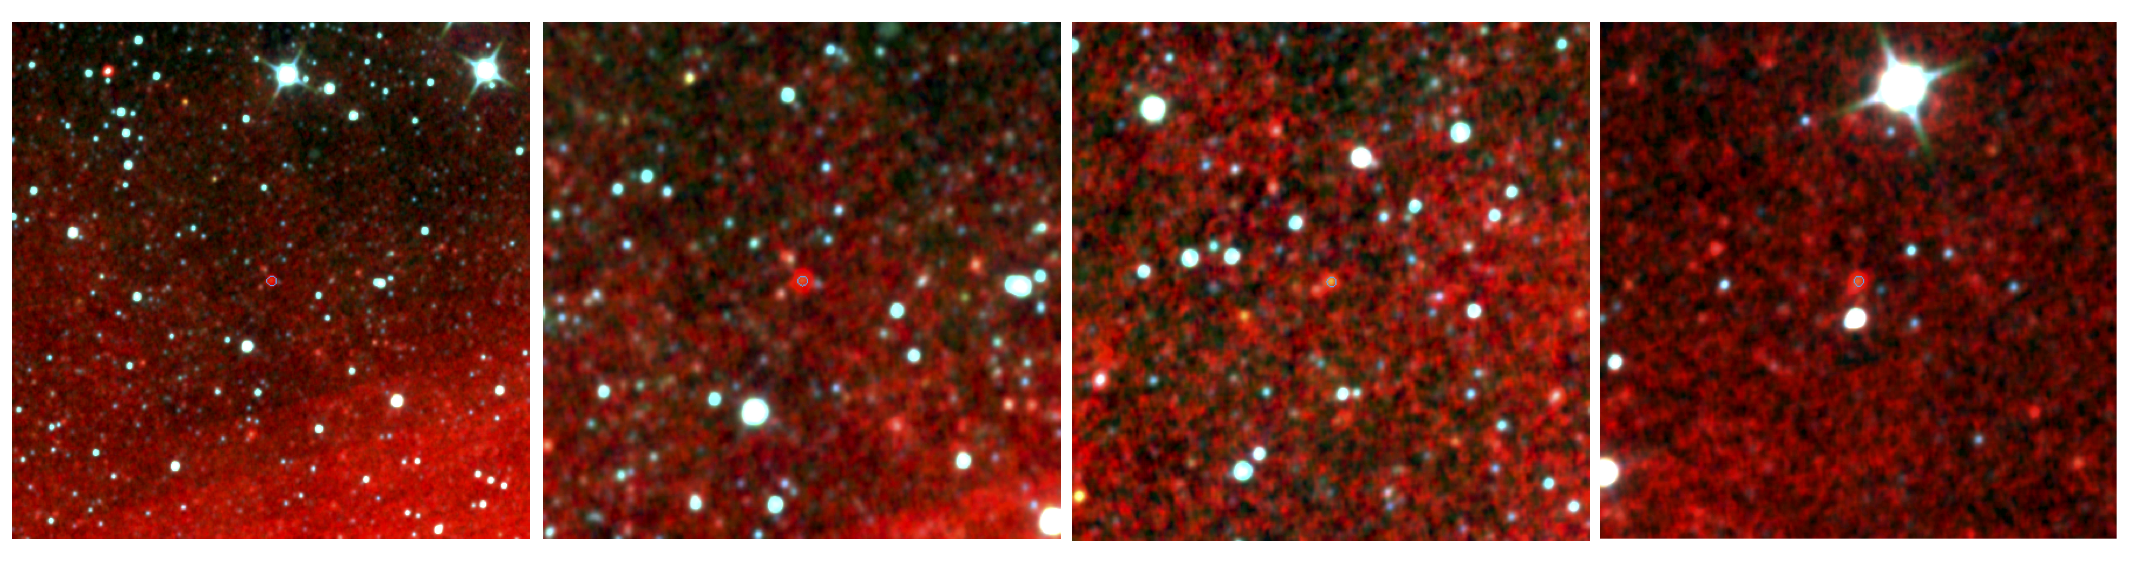
\includegraphics[height=6.0cm,width=17.8cm]{../Figures/ERQs_4inarow_crop.png}
%    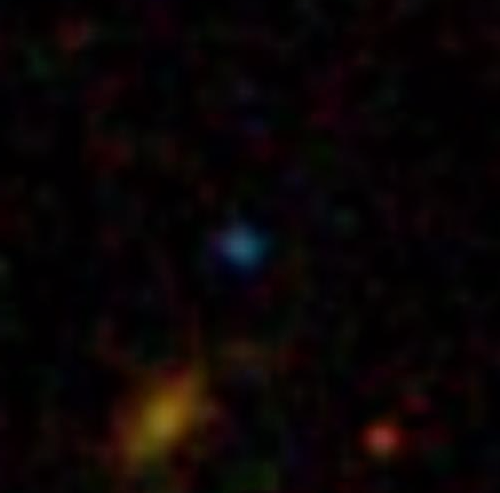
\includegraphics[height=7.0cm,width=7.0cm]{../Figures/ERQ_SDSS2_nolabel.png}
  %  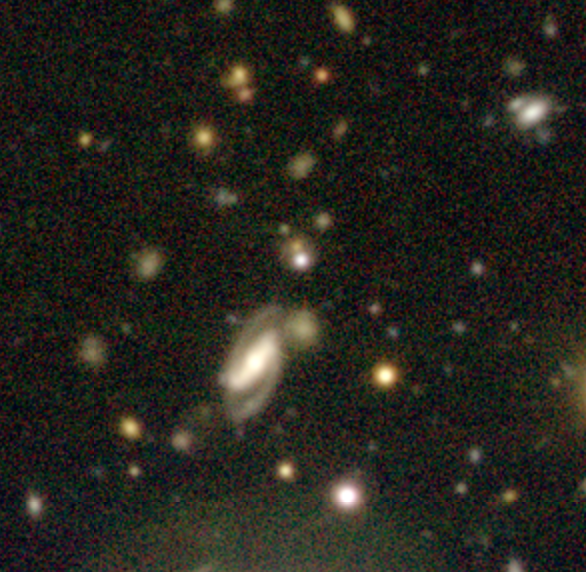
\includegraphics[height=7.0cm,width=7.0cm]{../Figures/ERQ_HSC1.png}
    \vspace{-10pt}
    \caption{
      % \small
      \footnotesize
      % \scriptsize
      % \tiny
      WISE 3.4, 4.6 and 12$\mu {\rm m}$ image of a $z=2.5$ 
      extremely red quasars, selected on their $r-[22]$ colour. This object
      has a 22$\mu$m flux indicative of $L_{IR} \gtrsim 10^{13.5} L_{\odot}$, 
      and one interpretation could be we are witnessing the
      ``birth'' of an unobscured QSO.  
 {\bf Why can I only get one figure on this page????!!!}
}
    \vspace{-14pt}
    \label{figtest-fig}
  \end{center}
\end{figure}

\hspace{-7.5cm}
\begin{figure}[h]
  \begin{center}
    \hspace{-0.5cm}
    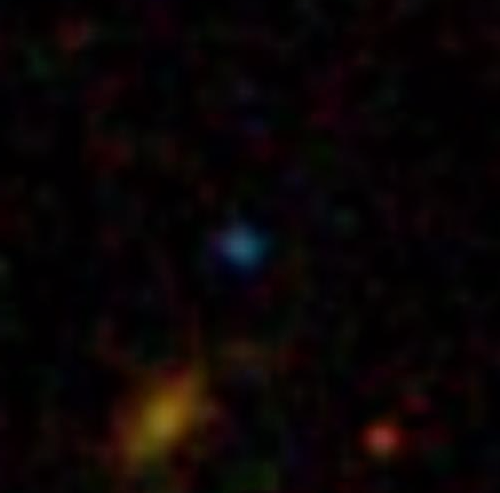
\includegraphics[height=7.0cm,width=7.0cm]{../Figures/ERQ_SDSS2_nolabel.png}
    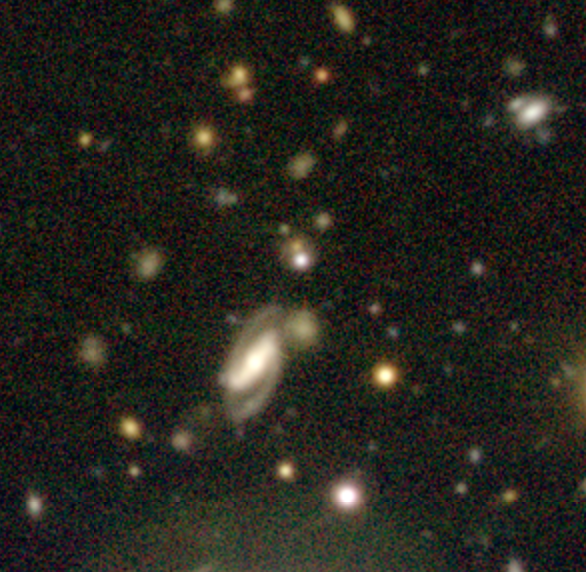
\includegraphics[height=7.0cm,width=7.0cm]{../Figures/ERQ_HSC1.png}
    \vspace{-10pt}
    \caption{
      % \small
      \footnotesize
      % \scriptsize
      % \tiny
      SDSS {\it (left)} and HSC {\it (right)} imaging of ERQ
      J2323-0100.  The gorgeous HSC data reveal a potential companion galaxy
      to J2323-0100 at the 11 o'clock position.}
    \vspace{-14pt}
    \label{figtest-fig}
  \end{center}
\end{figure}



\hspace{-2.5cm}
\begin{figure}[h]
  \begin{center}
    \hspace{-0.5cm}
    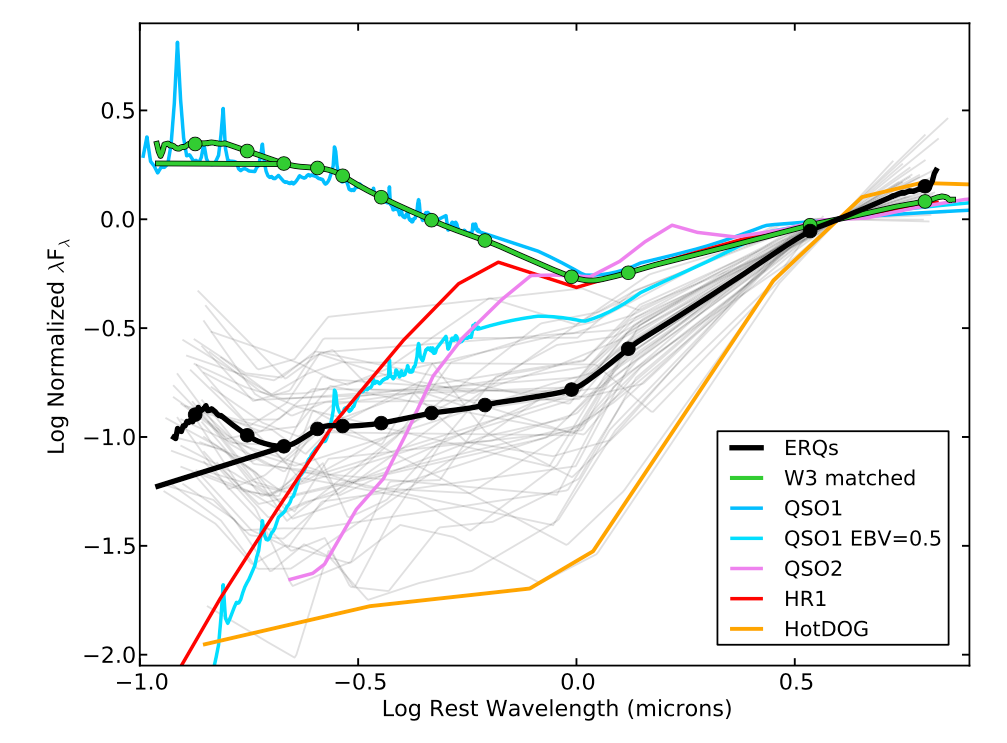
\includegraphics[height=7.0cm,width=7.0cm]{../Figures/Hamann2017_Fig16_SEDs.png}
%    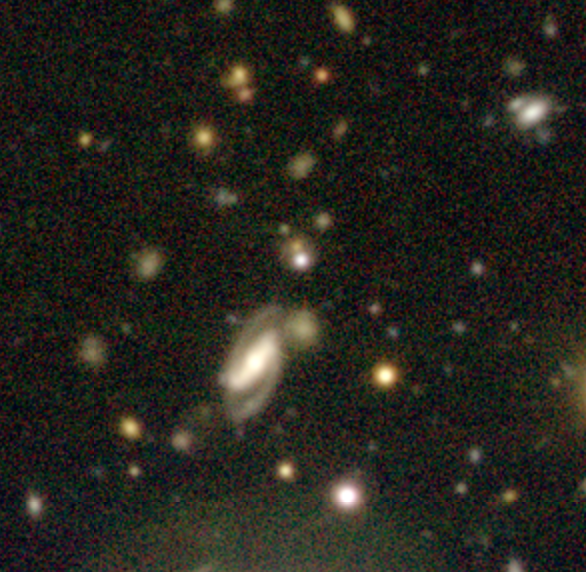
\includegraphics[height=7.0cm,width=7.0cm]{../Figures/ERQ_HSC1.png}
    \vspace{-10pt}
    \caption{
      % \small
      \footnotesize
      % \scriptsize
      % \tiny
      {\it (left)} From Hamann et al., 2017, the normalized median
      SEDs for Type 1 non-BALs in the core ERQ sample (black curve) plus
      blue quasars matched to the core ERQs in W3 magnitude (green curve) as
      in Fig. 8, the Type 1 quasar template QSO1 with and without reddening
      equal to $E(B − V) = 0.5$ (light blue, from Polletta et al. 2007), a
      typical Type 2 quasar (QSO2) from Mateos et al. (2013, purple), a
      typical heavily reddened Type 1 quasar (HR1) from Banerji et
      al. (2013), and a typical HotDOG from Tsai et al. (2015). The light
      grey curves are SEDs of individual core ERQs.
    }
    \vspace{-14pt}
    \label{figtest-fig}
  \end{center}
\end{figure}









\clearpage
%%%%%%%%%%%%%%%%%%%%%%%%%%%%%%%%%%%%%%%%%%%%%%%%%%%%%%%%%%%%%%%%%%%%%%%%%%%

%   3a. TECHNICAL DESCRIPTION 
%        (was previously  DESCRIPTION OF THE OBSERVATIONS)
%        (see https://jwst-docs.stsci.edu/display/JSP/JWST+DD+ERS+Proposal+Preparation)
%
%
\describeobservations   % Do not delete this command.
% Enter your description of the observations.
%%%%%%%%%%%%%%%%%%%%%%%%%%%%%%%%%%%%%%%%%%%%%%
%%
%%    D e s c r i p t i o n    o f     t h e      O b s e r v a t i o n s  : 
%%
%%%%%%%%%%%%%%%%%%%%%%%%%%%%%%%%%%%%%%%%%%%%%%

Describe the targets and observational modes to be used. Quantitative
estimates must be provided of the accuracy required to achieve key
science goals. Proposers must demonstrate that all observations can
execute in the first 5 months of Cycle 1 (planned to be from April to
August 2019), and that a substantive subset of the observations are
accessible in the first 3 months. This description should also include
the following::

\begin{enumerate}[label=\alph*]
    \item{Plan for Alternative Targets: As described in JWST DD ERS
        Special Observational Policies, proposers should qualitatively
        describe the availability of alternate targets and the process used to
        identify those targets should the start of science observations be
        delayed.  Robust ERS programs involve science investigations that can
        be performed with a variety of different targets and observations. }
      
    \item{Special Observational Requirements (if any): Justify any
        special scheduling requirements, e.g., time-critical observations.}

    \item{Justification of Coordinated Parallels (if any): Proposals
        that include coordinated parallel observations should provide a
        scientific justification for and description of the parallel
        observations. It should be clearly indicated whether the parallel
        observations are essential to the interpretation of the primary
        observations or the science program as a whole, or whether they
        address partly or completely unrelated issues. The parallel
        observations are subject to scientific review, and can be rejected
        even if the primary observations are approved.}

    \item{Justification of Duplications (if any): as detailed in the JWST
        DD ERS Proposal Policies and the JWST Duplicate Observations Policy,
        observations taken as part of the DD ERS program cannot duplicate
        those specified for the GTO Cycle 1 Reserved Observation Catalog
        (planned for release on June 15, 2017). Any duplicate observations
        must be explicitly justified.}
\end{enumerate}


\clearpage
\begin{tabular}{||  l|l|l|l|l ||}
\hline\hline
 &&&& \\
Object Name (SDSS)        & J0834+0159         &  J1232+0912          & J2215-0056        & J2323-0100 \\
 &&&& \\
\hline
 &&&& \\
Object R.A.                      & 08:34:48.48         & 12:32:41.73           & 22:15:24.00          & 23:23:26.17     \\
object declination           & $+$01:59:21.1     & $+$09:12:09.3      & $-$00:56:43.8      & $-$01:00:33.1  \\
$r$-band AB magnitude   & 21.20$\pm$0.05  & 21.11$\pm$ 0.05  & 22.27$\pm$0.12  & 21.62$\pm$ 0.08 \\  
Redshift $z_{\rm in}$        &  2.591                   &  2.381                    &  2.509                  &  2.356 \\  
CIV FWHM km s$^{-1}$   & 2863$\pm$65       & 4787$\pm$52       & 4280$\pm$112   & 3989$\pm$62 \\ 
\oiii\ FWHM erg s$^{-1}$ & 2811                      & 4971                     & 3057                    & 2625 \\ %% From Zam16
%\oiii FWHM erg s$^{-1}$ & ---                        & 5627                  & 3057                   & 2625 \\ %% From Alexan_the
Spectro-polarimertry       &   $\times$            &  $\surd$                &  $\surd$           & $\times$  \\
VLA data                          & ?                            &?                             & ?                        & ?  \\ 
ALMA  Band 6                  & tbc                        & $\surd$                & tbc                     & $\surd$  \\
 &&&& \\
JWST target visibility (Start) & 2019-04-01    & 2019-05-08    & 2019-05-22   & 2019-06-07  \\ 
JWST target visibility (End)  & 2019-05-07    & 2019-07-01     & 2019-07-15   & 2019-07-29   \\ 
 &&&& \\
\hline\hline
\end{tabular}


\hspace{-2.5cm}
\begin{figure}[h]
  \begin{center}
    \hspace{-0.5cm}
    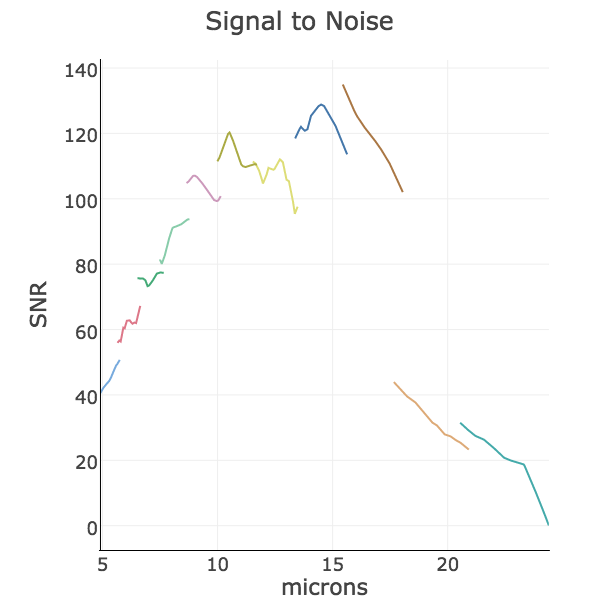
\includegraphics[height=7.0cm,width=7.0cm]{../Figures/current_wavelength_vsSNR.png}
    \vspace{-10pt}
    \caption{       \footnotesize}
    \vspace{-14pt}
    \label{figtest-fig}
  \end{center}
\end{figure}



%%%%%%%%%%%%%%%%%%%%%%%%%%%%%%%%%%%%%%%%%%%%%%%%%%%%%%%%%%%%%%%%%%%%%%%%%%%

%   3b. PLAN FOR ALTERNATIVE TARGETS
%       (see https://jwst-docs.stsci.edu/display/JSP/JWST+DD+ERS+Proposal+Preparation)
%
%
\alttargets   % Do not delete this command.
% Enter your plan for for alternative targets here.


%%%%%%%%%%%%%%%%%%%%%%%%%%%%%%%%%%%%%%%%%%%%%%%%%%%%%%%%%%%%%%%%%%%%%%%%%%%

%   3c. SPECIAL REQUIREMENTS
%        (see https://jwst-docs.stsci.edu/display/JSP/JWST+DD+ERS+Proposal+Preparation)
%
%
\specialreq             % Do not delete this command.
% Justify your special requirements here, if any.

%%%%%%%%%%%%%%%%%%%%%%%%%%%%%%%%%%%%%%%%%%%%%%%%%%%%%%%%%%%%%%%%%%%%%%%%%%%

%   3d. COORDINATED PARALLEL OBSERVATIONS
%        (see https://jwst-docs.stsci.edu/display/JSP/JWST+DD+ERS+Proposal+Preparation)
%
%
\coordinatedobs % Do not delete this command.
% Enter your coordinated parallel observing plans here, if any.

%%%%%%%%%%%%%%%%%%%%%%%%%%%%%%%%%%%%%%%%%%%%%%%%%%%%%%%%%%%%%%%%%%%%%%%%%%%

%   3e. JUSTIFY DUPLICATIONS
%        (see https://jwst-docs.stsci.edu/display/JSP/JWST+DD+ERS+Proposal+Preparation)
%
%
\duplications           % Do not delete this command.
% Enter your duplication justifications here, if any.



\clearpage
%%%%%%%%%%%%%%%%%%%%%%%%%%%%%%%%%%%%%%%%%%%%%%%%%%%%%%%%%%%%%%%%%%%%%%%%%%%

%   4. DATA PROCESSING AND ANALYSIS PLAN
%       (see https://jwst-docs.stsci.edu/display/JSP/JWST+DD+ERS+Proposal+Preparation)
%
%
\analysisplan % Do not delete this command.
% Describe the data processing and analysis plan here.
\section*{General Outline and Motvations Driving Data Processing \& Analysis}
Our ERQ ERS proposal is the first part of a multi-cycle proposal
project and plan.  As such, we are {\it already highly motivated to
produce the data processing tools, codes, documentation and identify
the critical science-enabling products well in advance of the release
of the Cycle 2 Call for Proposals (September 2019).}

\smallskip \smallskip
\noindent
Our Science-Enabling Products team consists of four main parts::
\begin{itemize}
    \item ``Core Coders''; 
    \item  Wedsite and {\tt readthedocs} Writers; 
    \item Observational Follow-up; 
    \item Senior members of staff, able to supply students/ ask for funding; 
    \item Operating akin to a steering committee; 
\end{itemize}


\section*{ERS ERQ Science Enabling Products}
{\tt mrs\_analyzer} is  a Python module for analyzing MRS data; 
{\tt mrsfringe} is a Python module for mitigating MRS fringing issues; 

\smallskip \smallskip
\noindent
And will integrate with...
\href{https://github.com/STScI-JWST}{\tt https://github.com/STScI-JWST} \\
see e.g. 
{\tt https://github.com/STScI-JWST/jwst/blob/master/jwst/mrs\_imatch/mrs\_imatch\_step.py}



\section*{Delivery Schedule for Science-Enabling Products.} 
Here we give the delivery schedule for science-enabling products. 
Proposals must present a delivery schedule for science-enabling products. A description of STScI pipeline data products, processing and analysis software, and their anticipated availability, will be provided by the May 2017 release of the final version of this Call for Proposals.  Proposers may consider multiple deliveries, with more advanced products provided over longer timescales. Proposals may include the collection, processing and analysis of ancillary data as part of an integrated DD ERS proposal.

\section*{Co-Investigators and Delivery of Science-Enabling Products.}
Co-Investigators, together with the PI (and any Co-PIs) comprise a core team with the responsibility of developing and delivering science-enabling products as described in the proposal, as well as carrying out selected key aspects of the science investigations.  A Co-I must have a well-defined, and generally sustained, continuing role in team activities, serve under the direction of the PI, or co-PI(s). Co-investigators may or may not receiving funding, pending eligibility, through the DD ERS program. 

\subsection{Dr. Nicholas Ross}
P.I. Dr. Nic Ross is a deep believer in delivering science-enabling
products, including datasets, catalogs, analysis codes, plots,
algorithms and where possible computational resources to the wide
astronomical community.  As such, the call for delivering
science-enabling products by the release of the Cycle 2 Call for
Proposals (September 2019) is fully inline with his scientific
practice.

\smallskip \smallskip
\noindent
Ross has being developing and buidling up his GitHub Repositories over
the last year or so, \href{https://github.com/d80b2t}{\tt
github.com/d80b2t} and indeed now does all his analysis and paper
writing on GitHub.

\smallskip \smallskip
\noindent
Ross will devote a considerable amount of his personal research time
(and due to his STFC ERF has 100\% FTE for research) to leading the
developement and timely prodcution of the ERS ERQ science-enabling
products.


\subsection{Dr. David Rosario} 
Co-PI Dr. David Rosario is awesome and also loves to write code. ;-)


\subsection{Prof. David Alexander} 
Prof. Alexander is an expert in high-$z$ obsured AGN.  He will use his
considerable {\it Spitzer IRS} expereince to help test our MIRI MRS
data-analysis toolkit.


\subsection{Dr. Rachael Alexandroff} 
Dr. Alexandroff is an leading expert on the ERQ population.  She will
bring to bear her now considerable and recent data analysis (long-slit
optical, polarimerty, radio) data analysis experience to build our
MIRI MRS data-analysis toolkit.


\subsection{Dr. Richard Bielby}

\iffalse
\subsection{Prof. Beth Biller}
Prof. Biller is an expert in infrared coronagraphic observations. 
While we do not intend to use the MIRI coronagraphs in this proposal, 
longer term observations would potentially involve observing the ERQs
with the Lyot or 4QPM if this became appropriate and technically feasible. 
\fi


\subsection{Prof. Niel Brandt}


\subsection{Dr. Rob Crain}
Dr. Rob Crain is a Royal Society University Research Fellow and will 
lead the theoretical team. 


\subsection{Prof. Xiaohui Fan}
Prof. Fan is a leader in surveys of high-redshift quasars and
reionization. He has extensive experience in studying quasars and
their host galaxies with {\it HST} and {\it Spitzer}.


\subsection{Prof. Fred Hamann}


\subsection{Prof. Dale Kocevski}
Prof. Kocevski is...
We are also asking for the appriopriate level of 
post-doctoroal support for Prof. Kocevski. 

\subsection{Prof. Linhua Jiang}


\subsection{Dr. Stephanie LaMassa}
Dr. LaMassa is currently at the STScI and is already involved with the
documentation efforts there. As such, Dr. LaMassa will help with those
efforts, along with writing code and potentially leading follow-up
where approriate. She will also be a natural link to the direct
efforts of the Space Telsecop Science Institute.


\subsection{Dr. Chelsea MacLeod}


\subsection{Dr. Ian McGreer}


\subsection{Prof. Brice Menard}	


\subsection{Dr. James Mullaney}


\subsection{Prof. Adam Myers}
Prof. Myers is an expert on the statistical analysis of reddened,
obscured and optically luminous quasars. He has co-authored many
well-cited publications on targeting quasars, quasar clustering,
high-redshift and unusual quasars, and quasars in the time
domain. Prof. Myers has made follow-up observations of quasars, and
other objects, at telescopes on five continents. His work has been
funded multiple times by the NSF and NASA, including via space
telescope programs such as those for {\it Chandra} and {\it Spitzer}. He has
served on time allocation committees for GALEX and the {\it HST}. 

\smallskip \smallskip
\noindent
Prof. Myers has also worked extensively in large survey
collaborations, often in formal management roles. He is an Architect
of SDSS-III and SDSS-IV, was the quasar target selection lead for the
SDSS-IV/eBOSS survey, is the Level 3 Target Selection Manager for the
Dark Energy Spectroscopic Instrument (DESI) and is the documentation
and website lead for the Legacy Surveys
(http://legacysurvey.org). {\it Prof. Myers is a strong advocate for
transparent and reproducible science. For example, as part of his work
on DESI, he has contributed over 10,000 lines of code to publicly
visible github repositories.}


\subsection{Dr. Jessie Runnoe}
Dr. Runnoe is an expert on quasar central engines at radio through
X-ray wavelengths.  Drawing on her vast observational experience, she
will contribute to the development of the MIRI MRS data-analysis
toolkit and assist with follow-up observations of the ERQ core sample.
She will be part of the Core Coding and Observational Follow-up
groups.

\subsection{Prof. Don Schneider}
Prof. Donald Schneider has been involved with the Sloan Digital Sky
Survey since its earliest design stages in the 1980s and has
considerable experience in preparing large datasets for community use,
via leading several editions of the SDSS Quasar Catalogs and
participating in the annual public Data Releases. Prof. Schneider will
be on the follow-up Observational team, obtaining time on the HET if
necessary.


\subsection{Prof. Tom Shanks}	


\subsection{Dr. John Stott}


\subsection{Prof. Michael  Strauss}


\subsection{Dr. Renske Smit}		


\subsection{Prof. Martin Ward}		


\subsection{Prof. Gillian Wright}


\subsection{Prof. Nadia Zakamsaka} 


\section*{Current Resources and inspirations}
\subsection*{The NASA Ames PAH IR Spectroscopic Database}
We will link to the NASA Ames PAH IR Spectroscopic Database:: \\
http://www.astrochem.org/pahdb/ \\
Bauschlicher et al, 2010, ApJS, 189, 341; Boersma et al, 2014, ApJS, 211, 8;  Mattioda et al., ApJS, in prep.\\

\subsection{PandExo: An Exoplanet ETC}
\href{https://natashabatalha.github.io/PandExo/}{\tt https://natashabatalha.github.io/PandExo/}

\subsection{The SMART Data Analysis Package for the Infrared Spectrograph1 on the Spitzer Space Telescope}
The SMART Data Analysis Package for the Infrared Spectrograph on the
Spitzer Space Telescope from S. J. U. Higdon,3 D. Devost,3
J. L. Higdon,3 B. R. Brandl,4 J. R. Houck,3 P. Hall,3 D. Barry,3
V. Charmandaris,3,5 J. D. T. Smith,6 G. C. Sloan,3 and J. Green7
Publications of the Astronomical Society of the Pacific, 116:975–984,
2004 October.





%%%%%%%%%%%%%%%%%%%%%%%%%%%%%%%%%%%%%%%%%%%%%%%%%%%%%%%%%%%%%%%%%%%%%%%%%%%





\end{document}          % End of proposal. Do not delete this line.
                        % Everything after this command is ignored.

